\section{Durchführung}
\label{sec:Durchführung}

Für die Untersuchung der Zeitabhängigkeit der Amplitude, wird die in Abbildung (5) dargestellte Schaltung verwendet.

\begin{figure}[H]
  \centering
  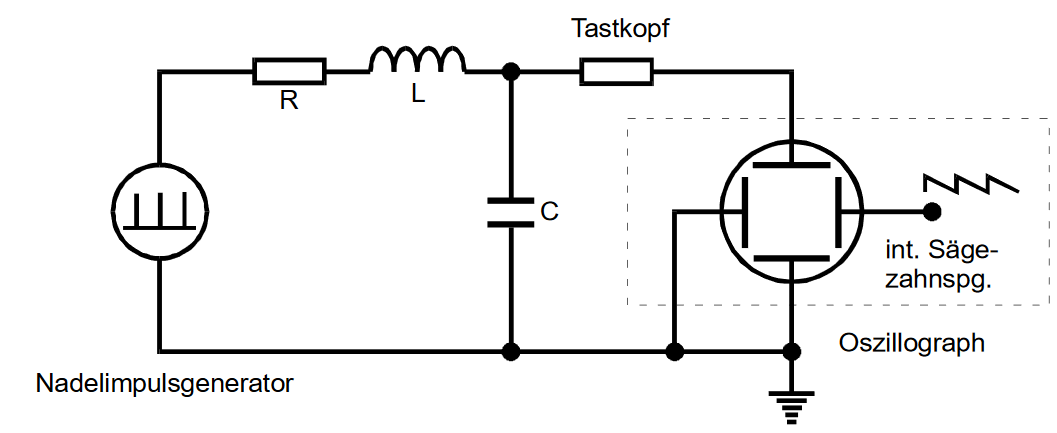
\includegraphics[height=5cm]{Schaltung1.png}
  \caption{Messschaltung zur Bestimmung der zeitabhängigen Amplitude. \cite[S. 11]{kent}}
\end{figure}
\noindent Um gedämpfte Schwingungen zu erzeugen, wird durch eine Rechteckspannung ein Impuls an den Schwingkreis gegeben.
Ein Tastkopf ist notwendig, um den Eingangswiderstand des Oszillographen verschwindend gering zu halten. 
Es werden für zehn verschiedene Zeiten die Amplitude am Oszilloskop abgelesen und damit der effektive Dämpfungswiderstand ermittelt.
Die gegebenen Daten für die Bauteile sind durch 
\begin{align*}
&L = 16,78 \pm 0,09 \, \si{\milli\henry} \\
&C = 2,066 \pm 0,006 \, \si{\nano\farad} \\
&R_1 = 67,2 \pm 0,2 \, \si{\ohm} \\
&R_2 = 682 \pm 1 \, \si{\ohm} \\
\end{align*}
gegeben. Bei diesem Messvorgang wird der Widerstand $R_1$ genommen.


\noindent Es wird der Dämpfungswiderstand für den aperiodischen Grenzfall bestimmt. Das geschieht durch Aufbau der Schaltung in Abbildung (6).
Der regelbare Widerstand wird auf seinen Maximalwert gestellt und dann runter gedreht. Dabei wird der zeitliche Verlauf der Spannung auf dem Oszillosgraph 
beobachtet, denn stellt sich ein Überschwingen ein, muss der Widerstand wieder höher gestellt werden. Wenn kein Überschwingen mehr
auftritt, wird der Wert für den Widerstand abgelesen.
\begin{figure}[H]
  \centering
  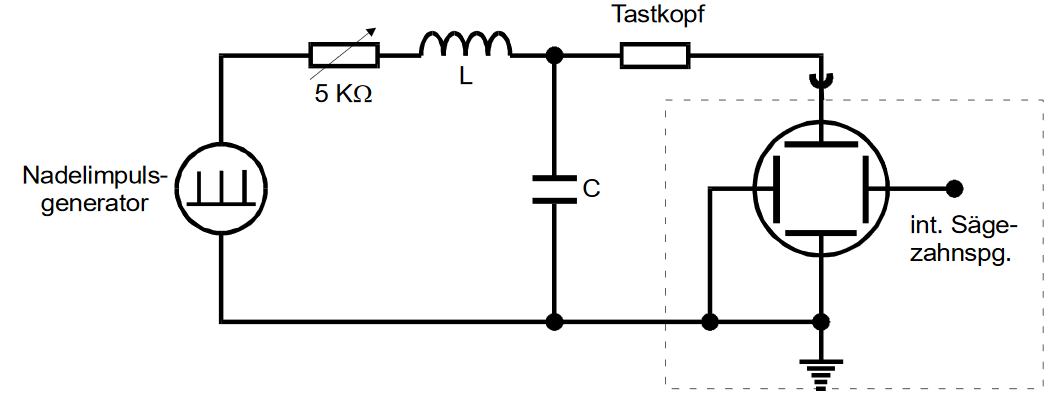
\includegraphics[height=5cm]{Schaltung2.png}
  \caption{Messschaltung für den aperiodischen Grenzfall. \cite[S. 12]{kent}}
\end{figure}

\noindent Soll die Frequenzabhängigkeit der Kondensatorspannung untersucht werden, wird der Schaltkreis wie in Abbildung (7) aufgebaut.
Es wird diesmal eine Sinusspannung angelegt. Da der dort zu sehende Tastkopf einen Frequenzgang besitzt, muss die Erregerspannung $U_0$ in Abhängigkeit der Frequenz gemessen werden.
Es werden für folgende Intervalle Erregerspannung und Kondensatorpannnung gemessen: 2 \si{\kilo\hertz} bis 22 \si{\kilo\hertz} in 2 \si{\kilo\hertz} Schritten, 22 \si{\kilo\hertz} bis 32 \si{\kilo\hertz} in 1 \si{\kilo\hertz} Schritten,
32 \si{\kilo\hertz} bis 52 \si{\kilo\hertz} in 2 \si{\kilo\hertz} Schritten, und daraus der Quotient gebildet. Es wird der Widerstand  $R_2$ benutzt.
\begin{figure}[H]
  \centering
  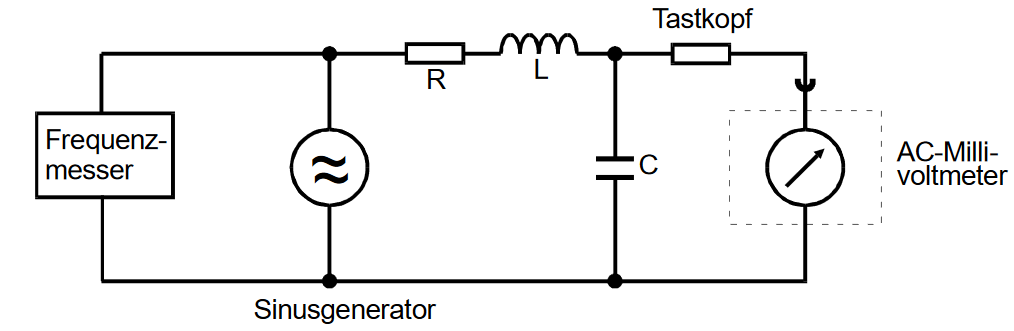
\includegraphics[height=5cm]{Schaltung3.png}
  \caption{Messschaltung zur Bestimmung der frequenzabhängigen Amplitude. \cite[S. 13]{kent}}
\end{figure}


\noindent Im letzten Versuchsteil wird die Frequenzabhängigkeit der Phase ermittelt. Die Schaltung ist in Abbildung (8) dargestellt.
Es wird der zeitliche Abstand $a$ der Nulldurchgänge von Kondensatorspannung und Erregerspannung gemessen, wie in Abbildung (9) dargestellt.
Die außerdem benötigte Periodendauer wird durch die Frequenz bestimmt, die vorher schon gemessen wurde.
\begin{figure}[H]
  \centering
  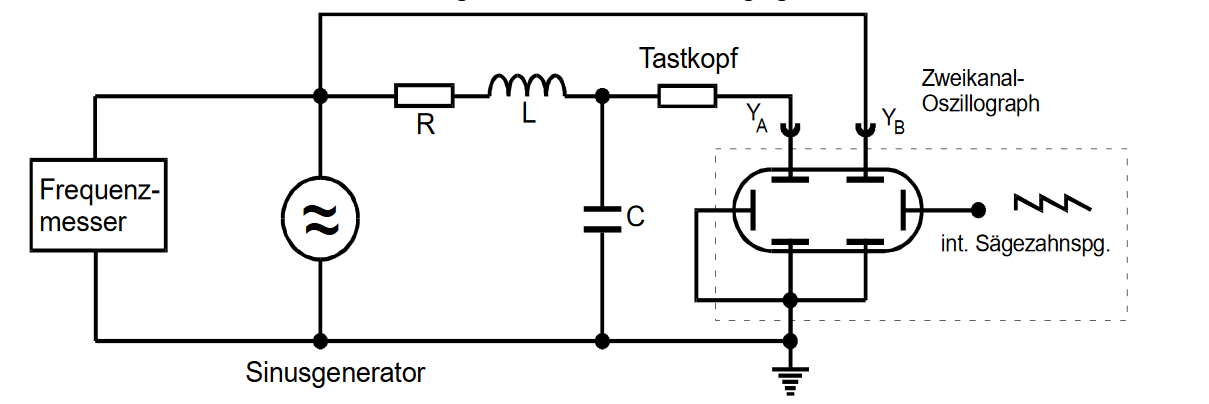
\includegraphics[height=5cm]{Schaltung4.png}
  \caption{Messschaltung zur Bestimmung der frequenzabhängigen Phase. \cite[S. 13]{kent}}
\end{figure}
\begin{figure}[H]
  \centering
  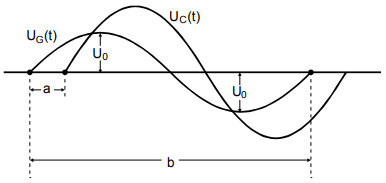
\includegraphics[height=5cm]{phi.png}
  \caption{Bestimmung der Nulldurchgänge. \cite[S. 7]{l}}
\end{figure}

